% Full 2 body problem
\chapter{The Full 2-Body Problem}
\label{F2BP}
\graphicspath{{chapter-4/Images/}}

\section{Introduction}
This chapter presents the coupled rotational and orbital motion of a binary asteroid system wherein both the bodies are modeled as a polyhedron and are under the influence of their mutual gravitational potential. The dynamical equations presented here are applicable to any binary asteroid system with individual asteroids having any arbitrary shape and mass distribution. As mentioned in \Cref{intro} that the initial goal of this literature study was to study the motion of a spacecraft around a binary asteroid system, which was inspired by a future mission called \gls{AIDA} (see \Cref{aida}) wherein one of the spacecrafts in the joint \gls{NASA} \gls{ESA} mission will be orbiting around the binary asteroid Didymos. This is the reason why in this chapter we present the theory to understand the dynamical system around a binary asteroid system.

But before we begin with discussing the motion for two polyhedrons, we will briefly look at (relatively) lower-fidelity binary asteroid models namely the sphere-ellipsoid and ellipsoid-ellipsoid systems.

\subsection{Sphere-Ellipsoid Binary System}
In this full two-body problem formulation, the primary is modeled as an ellipsoid with semi-major axes $\alpha$, $\beta$, and $\gamma$ and the secondary is modeled as a sphere. Both bodies are uniform with constant densities. The geometry of the problem is given in \Cref{fig:se} \cite{chappaz}:
%
\begin{figure}[h]
\centering
\captionsetup{justification=centering}
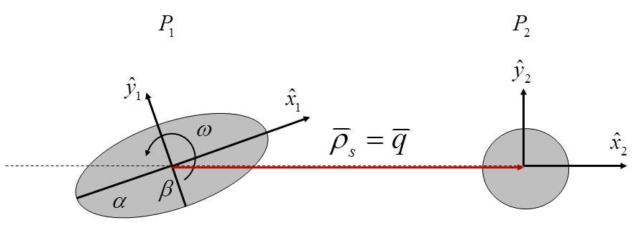
\includegraphics[scale=0.7]{se.png}
\caption{Geometry of sphere-ellipsoid binary system \cite{chappaz}.}
\label{fig:se}
\end{figure}
\FloatBarrier
%
The non-dimensional equations of motion for this system, i.e. for the sphere around the ellipsoid, are given as follows \cite{chappaz}:
\begin{equation}
\begin{aligned}
\ddot{\rho_s} + 2\omega \times \dot{\rho_s} + \omega \times (\omega \times \rho_s) + \dot{\omega} \times \rho_s &= \frac{\partial U_{e1}}{\partial \rho_s} \\
I \cdot \dot{\omega} + \omega \times I \cdot \omega &= -\mu \rho_s \times \frac{\partial U_{e1}}{\partial \rho_s}
\end{aligned}
\end{equation}
%
These equations are defined in a rotating frame fixed to the ellipsoid. The term $\rho_s$ is the non-dimensional position vector of the centre of mass of the sphere with respect to the ellipsoid as can be seen in \Cref{fig:se}; $\omega$ is the angular rate of the ellipsoid; $I$ is the inertia dyadic for the ellipsoid; $U_{e1}$ represents the gravitational potential of the ellipsoid \cite{chappaz}.

\subsection{Ellipsoid-Ellipsoid Binary System}
In this form of full two-body problem, both the asteroids are modeled as triaxial ellipsoids. It is assumed that both bodies are orbiting each other in a coplanar and equatorial orbit. The dynamics of the mutual orbit is then described by four degrees of freedom; one distance and three angles. One of the angles, $\theta$, defines the only rotation existing between the inertial and rotating frame of reference about the $z$-axis. The two other angles define the rotation angle of the two ellipsoids about the inertial $z$-axis, namely $\phi_1$ and $\phi_2$. The distance as a degree of freedom is basically the seperation between the centres of the two ellipsoids. The geometry for this binary formulation is given in \Cref{fig:ee} \cite{chappaz}. Note that the spacecraft is included in \Cref{fig:ee} only as an illustration and serves no purpose in this chapter since the dynamics of the spacecraft around the binary system will not be modeled here. The figure was added unaltered since it was sourced from a published paper.
%
\begin{figure}[h]
\centering
\captionsetup{justification=centering}
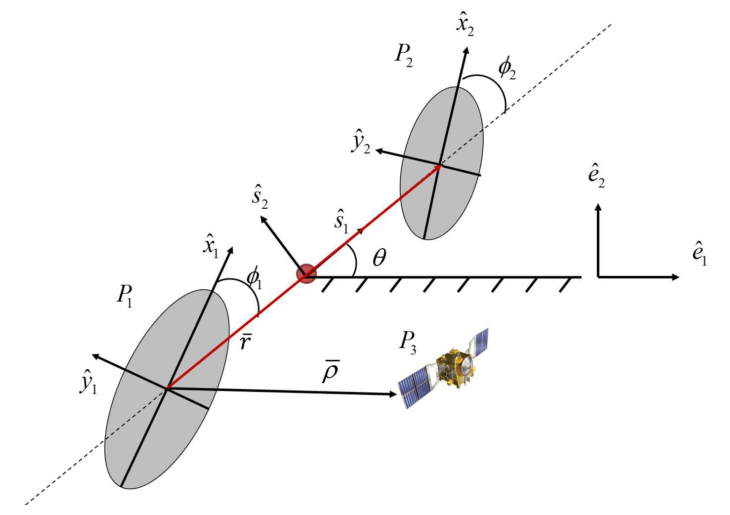
\includegraphics[scale=0.7]{ee.png}
\caption{Geometry of ellipsoid-ellipsoid binary system \cite{chappaz}. Note that the spacecraft is included here only as an illustration and the dynamics of it around the binary system have not been included in the equations of motion since this chapter is concerned only with the two-body problem.}
\label{fig:ee}
\end{figure}
\FloatBarrier
%
The equations of motion for the system are given as follows \cite{chappaz}:
\begin{equation}
\begin{aligned}
\ddot{r} &= \dot{\theta} r - \frac{1}{m} V_r \\
\ddot{\phi_1} &= -\left(1 + \frac{mr^2}{I_{1_z}} \right) \frac{1}{mr^2} V_{\phi_1} - \frac{1}{mr^2} V_{\phi_2} + 2 \frac{\dot{r} \dot{\theta}}{r} \\
\ddot{\phi_2} &= -\left(1 + \frac{mr^2}{I_{2_z}} \right) \frac{1}{mr^2} V_{\phi_2} - \frac{1}{mr^2} V_{\phi_1} + 2 \frac{\dot{r} \dot{\theta}}{r} \\
\ddot{\theta} &= \frac{1}{mr^2}(V_{\phi_1} + V_{\phi_2}) - 2 \frac{\dot{r} \dot{\theta}}{r}
\end{aligned}
\end{equation}
%
where $m$ denotes the reduced mass of the two bodies in the system as $m = \frac{m_1 m_2}{m_1 + m_2}$; $V$ is the potential energy (for a complete definition the reader should refer \cite{chappaz}) and the subscripts denote against what the partial differentiation of $V$ takes place; $I_{1_z}$ and $I_{2_z}$ denote the moment of inertia for the two bodies about the z-axis.

This was an introduction to the different ways in which earlier works have tried to model a binary system. The reader should refer to \cite{chappaz} to get more insight into these topics. We will now begin with describing the mutual potential formulation for a binary polyhedron system, and after that the force and the torque equations shall be presented which basically describe the coupled dynamics of the binary asteroid system.

\section{Mutual Potential Formulation for Two Polyhedrons}
\label{mutual_pot}
Let's begin with defining the underlying geometry that is used to build up the expression for the mutual potential. Each polyhedron is segmented into a collection of tetrahedrons called simplices. One of the vertices of each simplex is placed at the centroid of the polyhedron. The remaining three vertices form a triangular facet of the polyhedron. The position vectors are defined in an inertial reference frame, unless stated otherwise. We will denote the two asteroids with symbols \textit{A} and \textit{B}. The position vector to the centroid of body \textit{A} is defined as $\mathbf{A} = (x_A, y_A, z_A)$ and the position vector for a differential volume element \textit{dA} in \textit{A} is defined by $\mathbf{a} = (x_a, y_a, z_a)$, and in body-fixed frame the same is defined by $\mathbf{a}-\mathbf{A} = (\Delta x_a, \Delta y_a, \Delta z_a)$. Similar definitions also apply for a second body \textit{B} \cite{werner_poly}. These vectors can be visualized in \Cref{fig:poly1}.
%
\begin{figure}[h]
\centering
\captionsetup{justification=centering}
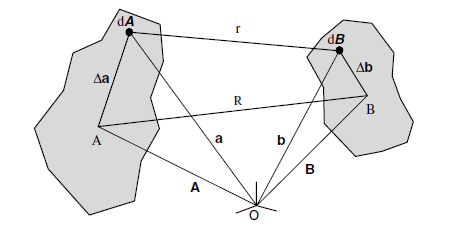
\includegraphics[scale=0.7]{poly1.png}
\caption{Vectors \textbf{a} and \textbf{b} denote the inertial position of the two differential volume elements, seperated from each other by a distance \textit{r}. Vectors \textbf{A} and \textbf{B} denote the inertial position of the two-body centroids, seperated by a distance \textit{R} \cite{werner_poly}.}
\label{fig:poly1}
\end{figure}
\FloatBarrier
%
The distance between the differential volumes is defined as follows \cite{werner_poly}:
\begin{align}
\label{r_def1}
r^2 &= (x_a - x_b)^2 + (y_a - y_b)^2 + (z_a - z_b)^2\\
\label{r_def2}
r^2 &= [(x_A - x_B) + (\Delta x_a - \Delta x_b)]^2 + [(y_A - y_B) + (\Delta y_a - \Delta y_b)]^2 + [(z_A - z_B) + (\Delta z_a - \Delta z_b)]^2
\end{align}
%
Following are the definition of two more vectors that will help in simplifying the notations \cite{werner_poly}:
\begin{align}
\mathbf{R} &\equiv (x_A - x_B, y_A - y_B, z_A - z_B)\\
\mathbf{h} &\equiv (\Delta x_a - \Delta x_b, \Delta y_a - \Delta y_b, \Delta z_a - \Delta z_b)
\end{align}
%
where their norms are obtained by scalar dot products as $R^2 = \mathbf{R} \cdot \mathbf{R}$ and $h^2 = \mathbf{h} \cdot \mathbf{h}$. Then 'r' from \Cref{r_def1} and \Cref{r_def2} can be redefined as \cite{werner_poly}:
\begin{align}
\label{r_def3}
r^2 &= (\mathbf{R} + \mathbf{h}) \cdot (\mathbf{R} + \mathbf{h}) \\
r^2 &= R^2 + h^2 + 2\mathbf{R} \cdot \mathbf{h}
\end{align}
%
The mutual potential is obtained by evaluating a pair of iterated integrals over the entire volume of the two bodies \textit{A} and \textit{B} \cite{werner_poly}:
\begin{equation}
\label{u_def1}
U \equiv \int \int \int_A \text{ } \int \int \int_B \frac{1}{r} dB \text{ } dA
\end{equation}
%
The above equation can also be rewritten in terms of the tetrahedral simplices \textit{a} and \textit{b} from the two bodies as follows \cite{werner_poly}:
\begin{equation}
\label{u_def2}
U = \sum_{a\in A} \text{ } \sum_{b\in B} \int \int \int_a \text{ } \int \int \int_b \frac{1}{r} db \text{ } da
\end{equation}
%
The series expansion of the term $(1/r)$ using Legendre polynomials (shown here until order 3) is given as \cite{werner_poly}:
\begin{equation}
\label{r_exp}
\frac{1}{r} = \left[\frac{1}{R}\right] + \left[\frac{-\mathbf{R} \cdot \mathbf{h}}{R^3}\right] + \left[\frac{-h^2}{2R^3} + \frac{3(\mathbf{R} \cdot \mathbf{h})^2}{2R^5}\right] + \left[\frac{3h^2(\mathbf{R} \cdot \mathbf{h})}{2R^5} - \frac{5(\mathbf{R} \cdot \mathbf{h})^3}{2R^7}\right]
\end{equation}
%
A change of variables from (x,y,z) to barycentre formulation (u,v,w) is performed to carry out the integration in \Cref{u_def2} \cite{werner_poly}. The vertex coordinates for a given simplex 'a' of body \textit{A} (similar definitions apply for simplex b of body \textit{B} as well) is given as \cite{werner_poly}:
\begin{align}
(x_1^a, y_1^a, z_1^a) &= (x_A,y_A,z_A) + (\Delta x_1^a, \Delta y_1^a, \Delta z_1^a)\\
(x_2^a, y_2^a, z_2^a) &= (x_A,y_A,z_A) + (\Delta x_2^a, \Delta y_2^a, \Delta z_2^a)\\
(x_3^a, y_3^a, z_3^a) &= (x_A,y_A,z_A) + (\Delta x_3^a, \Delta y_3^a, \Delta z_3^a)
\end{align}
%
The coordinates of any vertex for a simplex \textit{a} (and similarly for \textit{b}) in terms of the barycentre coordinates can be rewritten as \cite{werner_poly}:
\begin{equation}
\begin{bmatrix}
x_a\\
y_a\\
z_a
\end{bmatrix}
=
\begin{bmatrix}
x_A\\
y_A\\
z_A
\end{bmatrix}
+
\begin{bmatrix}
\Delta x_1^a & \Delta x_2^a	& \Delta x_3^a\\
\Delta y_1^a & \Delta y_2^a	& \Delta y_3^a\\
\Delta z_1^a & \Delta z_2^a	& \Delta z_3^a
\end{bmatrix}
\begin{bmatrix}
u_a\\
v_a\\
w_a
\end{bmatrix}
\end{equation}
%
where $(u_a, v_a, w_a)$ are the barycentre coordinates for simplex \textit{a} such that $0 \leq (u_a,v_a,w_a, u_a+v_a+w_a) \leq 1$ \cite{werner_poly}. The change of variables for integration requires introducing a certain Jacobian determinant which is described in the following equation \cite{werner_poly}:
\begin{equation}
\label{Tmatrix}
T_a
=
det
\begin{bmatrix}
\Delta x_1^a & \Delta x_2^a	& \Delta x_3^a\\
\Delta y_1^a & \Delta y_2^a	& \Delta y_3^a\\
\Delta z_1^a & \Delta z_2^a	& \Delta z_3^a
\end{bmatrix}
\end{equation}
%
A similar definition applies for $T_b$. The change to barycentre variables transforms each simplex \textit{a} and \textit{b} into a standard simplex form \textit{a'} and \textit{b'} respectively with barycentre coordinates as (0,0,0), (0,0,1), (0,1,0), and (1,0,0) \cite{werner_poly}. Using this new information, the mutual potential expression from \Cref{u_def2} changes to the following form \cite{werner_poly}:
\begin{equation}
\label{u_def3}
U = \sum_{a\in A} \text{ } \sum_{b\in B} T_aT_b \int \int \int_{a'} \text{ } \int \int \int_{b'} \frac{1}{r} db' \text{ } da'
\end{equation}
%
Now we are going to define some intermediate terms that will also be present in the final expression of the mutual potential. The reader is advised that from here onwards, unless stated otherwise, we adopt tensor notation and the Einstein summation convention and hence the reader should not attribute any significance to the distinction of superscript and/or subscript indices \cite{werner_poly}.

The coordinates to the vertices of the simplices \textit{a} and \textit{b}, relative to each body's centroid, are defined using three 6-element vectors (negative weight is given to the vertices of simplex \textit{b}) as follows \cite{werner_poly}:
\begin{align}
\label{x_tensor}
\mathbf{x}^i &\equiv [\Delta x_1^a, \Delta x_2^a, \Delta x_3^a, -\Delta x_1^b, -\Delta x_2^b, -\Delta x_3^b]\\
\label{y_tensor}
\mathbf{y}^i &\equiv [\Delta y_1^a, \Delta y_2^a, \Delta y_3^a, -\Delta y_1^b, -\Delta y_2^b, -\Delta y_3^b]\\
\label{z_tensor}
\mathbf{z}^i &\equiv [\Delta z_1^a, \Delta z_2^a, \Delta z_3^a, -\Delta z_1^b, -\Delta z_2^b, -\Delta z_3^b]
\end{align}
%
\Cref{x_tensor}, \Cref{y_tensor} and \Cref{z_tensor} are stacked to define a new 3x6 matrix as follows \cite{werner_poly}:
\begin{equation}
\label{v_tensor}
\mathbf{v}_j^i
\equiv
\begin{bmatrix}
\Delta x_1^a, \Delta x_2^a, \Delta x_3^a, -\Delta x_1^b, -\Delta x_2^b, -\Delta x_3^b\\
\Delta y_1^a, \Delta y_2^a, \Delta y_3^a, -\Delta y_1^b, -\Delta y_2^b, -\Delta y_3^b\\
\Delta z_1^a, \Delta z_2^a, \Delta z_3^a, -\Delta z_1^b, -\Delta z_2^b, -\Delta z_3^b
\end{bmatrix}
=
\begin{bmatrix}
\mathbf{x}_i\\
\mathbf{y}_i\\
\mathbf{z}_i
\end{bmatrix}_j
\end{equation}
%
We define another vector containing the barycenter variables \cite{werner_poly}:
\begin{equation}
\label{q_tensor}
\mathbf{q}_i \equiv [u_a, v_a, w_a, u_b, v_b, w_b]
\end{equation}
%
From \Cref{r_exp}, the terms $\mathbf{R} \cdot \mathbf{h}$ and $h^2$ can be expressed using the above newly defined vectors. We begin with defining $\mathbf{h}_j$ as follows \cite{werner_poly}:
\begin{align}
\mathbf{h}_j &= [\mathbf{q}_i \mathbf{x}^i, \mathbf{q}_i \mathbf{y}^i, \mathbf{q}_i \mathbf{z}^i]_j\\
\mathbf{h}_j &= \mathbf{q}_i \mathbf{v}_j^i
\end{align}
%
To clarify, we will expand one of the terms from the above equation:
\begin{equation}
\mathbf{q}_i \mathbf{x}^i = q_1x_1 + q_2x_2 + q_3x_3 + q_4x_4 + q_5x_5 + q_6x_6
\end{equation}
%
Next, we define the term $\mathbf{R} \cdot \mathbf{h}$ \cite{werner_poly}:
\begin{align}
\mathbf{R} \cdot \mathbf{h} &= \mathbf{R}^j \mathbf{h}_j\\
 &= \mathbf{R}^j \mathbf{q}_i \mathbf{v}_j^i\\
 &\equiv \mathbf{q}_i \mathbf{w}^i
\end{align}
%
where we have defined a 6-element vector $\mathbf{w}^i$ for convenience \cite{werner_poly}:
\begin{equation}
\label{w_tensor}
\mathbf{w}^i \equiv \mathbf{R}^j \mathbf{v}_j^i
\end{equation}
%
The individual terms of the vector $\mathbf{w}^i$ are defined as follows:
\begin{align*}
w^1 &= R^1v_1^1 + R^2v_2^1 + R^3v_3^1\\
w^2 &= R^1v_1^2 + R^2v_2^2 + R^3v_3^2\\
w^3 &= R^1v_1^3 + R^2v_2^3 + R^3v_3^3\\
& \vdots \\
w^6 &= R^1v_1^6 + R^2v_2^6 + R^3v_3^6
\end{align*}
%
Note we used Einstein's summation convention to get the above individual elements of $\mathbf{w}^i$. To clarify further, consider the 3x6 matrix as defined in \Cref{v_tensor}, then, for example, the terms $v_1^6, v_2^6, v_3^6$ are the first, second, and third-row elements in the $6^{th}$ column of the matrix. Finally, we define the $h^2$ term as follows \cite{werner_poly}:
\begin{align}
h^2 &= \mathbf{h}_k \mathbf{h}_k \\
&= \mathbf{q}_i \mathbf{v}_k^i \mathbf{q}_j \mathbf{v}_k^j\\
&= (\mathbf{q}_i \mathbf{q}_j)(\mathbf{x}^i\mathbf{x}^j + \mathbf{y}^i\mathbf{y}^j + \mathbf{z}^i\mathbf{z}^j)\\
&= \mathbf{q}_{ij} \mathbf{r}^{ij}
\end{align}
%
Where, we defined a rank 2 tensor $\mathbf{q}_{ij} = \mathbf{q}_i \mathbf{q}_j$ such that $\mathbf{q}_i$ will be a column vector and $\mathbf{q}_j$ will be a row vector. We have also defined another rank 2 tensor, $\mathbf{r}^{ij}$, as follows \cite{werner_poly}:
\begin{equation}
\mathbf{r}^{ij} \equiv \mathbf{x}^i\mathbf{x}^j + \mathbf{y}^i\mathbf{y}^j + \mathbf{z}^i\mathbf{z}^j
\end{equation}
%
where, for example, a certain element of the tensor $\mathbf{r}^{ij}$ will be defined as $r^{23} = x^2x^3 + y^2y^3 + z^2z^3$. Note that the numbers are indices and not powers. The terms $\mathbf{x}, \mathbf{y}, \mathbf{z}$ are as defined in \Cref{x_tensor}, \Cref{y_tensor} and \Cref{z_tensor} respectively. So basically, the term $h^2$ is obtained as:
\begin{equation}
h^2 = \mathbf{q}_{11} \mathbf{r}^{11} + \mathbf{q}_{12} \mathbf{r}^{12} + \mathbf{q}_{13} \mathbf{r}^{13} + \hdots + \mathbf{q}_{66} \mathbf{r}^{66}
\end{equation}
%
We have described all the necessary intermediate terms that we shall find in the mutual potential expression and without showing any further derivation steps, we present the final expression as follows (only until order three) \cite{werner_poly}:
\begin{equation}
\label{U_final_1}
U = \frac{G \rho_A \rho_B V_A V_B}{R} + G \sum_{a\in A} \text{ } \sum_{b\in B} \rho_a \rho_b T_a T_b \left( \left[- \frac{\mathbf{Q}_{ij}\mathbf{r}^{ij}}{2R^3} + \frac{3\mathbf{Q}_{ij} \mathbf{w}^i \mathbf{w}^j}{2R^5} \right] + \left[\frac{3\mathbf{Q}_{ijk} \mathbf{r}^{ij} \mathbf{w}^k}{2R^5} - \frac{5\mathbf{Q}_{ijk} \mathbf{w}^i \mathbf{w}^j \mathbf{w}^k}{2R^7}  \right]  \right)
\end{equation}
%
where the terms in the square brackets are the second and third-order terms, the first-order term vanishes because \textbf{A} and \textbf{B} are polyhedra centroids and expansion was centered at these centroids (see \cite{werner_poly} for the proof) and the order-zero term is depicted by the first term on the right-hand side of \Cref{U_final_1}. $V_A$ and $V_B$ are the volumes of the two bodies respectively, G is the universal gravitational constant, $\rho_A$ and $\rho_B$ are the total densities of the two bodies, $\rho_a$ and $\rho_b$ represent the density of each individual tetrahedral simplex. The \textbf{Q} are multi-rank tensors whose values (upto order 3) are given in \cite{werner_poly}.

A more generalized expression for the mutual potential (again, only till order 3 is shown here) can be presented as follows \cite{fahn_poly}:
\begin{equation}
\label{U_final_2}
U = G \sum_{a\in A} \text{ } \sum_{b \in B} \rho_a T_a \rho_b T_b \left(\left[\frac{\mathbf{Q}}{R} \right] + \left[-\frac{\mathbf{Q}_i \mathbf{w}^i}{R^3} \right] + \left[- \frac{\mathbf{Q}_{ij}\mathbf{r}^{ij}}{2R^3} + \frac{3\mathbf{Q}_{ij} \mathbf{w}^i \mathbf{w}^j}{2R^5} \right] + \left[\frac{3\mathbf{Q}_{ijk} \mathbf{r}^{ij} \mathbf{w}^k}{2R^5} - \frac{5\mathbf{Q}_{ijk} \mathbf{w}^i \mathbf{w}^j \mathbf{w}^k}{2R^7}  \right] \right)
\end{equation}
%

\section{Force terms for equations of motion from mutual potential derivatives}
\label{force_terms}
To compute the force acting on body \textit{A} from body \textit{B}, the mutual potential is differentiated with respect each component of the centroid coordinates of body \textit{A}. Similarly, the force acting on body \textit{B} is computed. We will again make use of tensor notation to depict the various vector terms \cite{fahn_poly}:
\begin{align}
\mathbf{F}_\theta^A &= \frac{\partial U}{\partial \mathbf{A}_\theta} \\
\mathbf{F}_\theta^B &= \frac{\partial U}{\partial \mathbf{B}_\theta}
\end{align}
%
where $\theta$ is just the tensor index. The above equations require us to differentiate the terms \textit{R} and $\textbf{w}^i$ on the right-hand side of \Cref{U_final_2}. The differentiated terms are shown as follows \cite{fahn_poly}:
\begin{align}
\label{R_diff}
\frac{\partial R}{\partial \mathbf{A}_\theta} &= -\frac{\mathbf{R}_\theta}{R}\\
\label{w_diff}
\frac{\partial \mathbf{w}^i}{\partial \mathbf{A}_\theta} &= -\mathbf{v}_\theta^i
\end{align}
%
where $\mathbf{v}_\theta^i$ is as defined in \Cref{v_tensor}. Let the terms in the square bracket on the right-hand side of \Cref{U_final_2} be denoted as $\hat{U}_0$, $\hat{U}_1$, $\hat{U}_2$, and $\hat{U}_3$. The partial derivatives of each of these terms is given as follows \cite{fahn_poly}:
\begin{equation}
\label{u0_diff}
\frac{\partial \hat{U}_0}{\partial \mathbf{A}_\theta} = \frac{\mathbf{Q} \mathbf{R}_\theta}{R^3}
\end{equation}
%
The vector $R_\theta$ is obtained as $\mathbf{B} - \mathbf{A}$ where \textbf{B} and \textbf{A} are the inertial coordinates of the centroids of the respective bodies.
\begin{equation}
\label{u1_diff}
\frac{\partial \hat{U}_1}{\partial \mathbf{A}_\theta} = -\frac{3\mathbf{Q}_i \mathbf{R}_\theta \mathbf{w}^i}{R^5} + \frac{\mathbf{Q}_i \mathbf{v}_\theta^i}{R^3}
\end{equation}
%
\begin{equation}
\label{u2_diff}
\frac{\partial \hat{U}_2}{\partial \mathbf{A}_\theta} = -\frac{3\mathbf{Q}_{ij} \mathbf{r}^{ij} \mathbf{R}_\theta}{2R^5} + \frac{15\mathbf{Q}_{ij} \mathbf{R}_\theta \mathbf{w}^i \mathbf{w}^j}{2R^7} - \frac{3\mathbf{Q}_{ij} \mathbf{w}^i \mathbf{v}_\theta^j}{R^5}
\end{equation}
%
\begin{equation}
\label{u3_diff}
\frac{\partial \hat{U}_3}{\partial \mathbf{A}_\theta} = \frac{15\mathbf{Q}_{ijk} \mathbf{r}^{ij} \mathbf{R}_\theta \mathbf{w}^k}{2R^7} - \frac{3\mathbf{Q}_{ijk} \mathbf{r}^{ij} \mathbf{v}_\theta^k}{2R^5} - \frac{35\mathbf{Q}_{ijk} \mathbf{R}_\theta \mathbf{w}^i \mathbf{w}^j \mathbf{w}^k}{2R^9} + \frac{15\mathbf{Q}_{ijk} \mathbf{w}^i \mathbf{w}^j \mathbf{v}_\theta^k}{2R^7}
\end{equation}
%
Thus the force acting on body \textit{A} is given as follows \cite{fahn_poly}:
\begin{equation}
\label{force_on_A}
\mathbf{F}_\theta^A = G \sum_{a \in A} \text{ } \sum_{b \in B} \rho_a T_a \rho_b T_b \left[\frac{\partial \hat{U}_0}{\partial \mathbf{A}_\theta} + \frac{\partial \hat{U}_1}{\partial \mathbf{A}_\theta} + \frac{\partial \hat{U}_2}{\partial \mathbf{A}_\theta} + \frac{\partial \hat{U}_3}{\partial \mathbf{A}_\theta} \right]
\end{equation}
%
From Newton's Law, we know that the force acting on body \textit{B} is the negative of that acting on body \textit{A}. The force term described by \Cref{force_on_A} is defined in the inertial reference frame, however sometimes it is easier to work with a body-fixed frame. Consider a frame fined to the centroid of body \textit{A}, then the relative position vector as expressed in this frame is given as \cite{fahn_poly}:
\begin{equation}
\label{r_bodyfix}
\mathbf{R} = P^T (\mathbf{B} - \mathbf{A})
\end{equation}
%
where $P^T$ is a transformation matrix that transforms a quantity in the inertial frame to the body-fixed frame. Expressed in the body-fixed frame, the relative force term can be expressed as follows \cite{fahn_poly}:
\begin{equation}
\label{F_rel}
\mathbf{F}_{rel} = \frac{\partial U}{\partial \mathbf{R}}
\end{equation}
%
Now we already have a function to compute $\partial U/ \partial \mathbf{B}$ which is:
\begin{equation}
\label{force on B}
\frac{\partial U}{\partial \mathbf{B}} = -\mathbf{F}_\theta^A
\end{equation}
%
We do not have to write a separate piece of code to evaluate \Cref{F_rel} as all we have to do is to substitute \textbf{R} from \Cref{r_bodyfix} as argument instead of \textbf{B} into the code for \Cref{force on B}. We can not use $\partial U/ \partial \mathbf{A}$ obviously because the body-fixed frame is attached to body \textit{A}.

\section{Torque terms for equations of motion from mutual potential derivatives}
\label{torque_terms}
Let's define \textit{P} as the matrix that maps from body-fixed frame of body \textit{A} to the inertial frame, and \textit{S} be the matrix mapping from the body-fixed frame of body \textit{B} to the inertial frame. One of the ways to get the torque expressions in the coupled dynamics is to take the partial derivative of the mutual potential \textit{U} with respect to either of the mapping matrices, \textit{P} or \textit{S}. By chain rule of differentiation, this will ultimately lead to the partial derivative of the \textbf{v} (see \Cref{v_tensor}) with respect to the mapping matrix \cite{fahn_poly}. We shall redefine the format of writing the tensor \textbf{v} from \Cref{v_tensor} by making use of the aforementioned transformation matrices as follows \cite{fahn_poly}:
\begin{equation}
\label{v_ten}
\mathbf{v} =[P[\Delta r^{a1}, \Delta r^{a2}, \Delta r^{a3}], -S[\Delta r^{b1}, \Delta r^{b2}, \Delta r^{b3}]]
\end{equation}
%
where each $\Delta r^{(a,b)i}$ represents a column vector depicting the coordinates of the vertex ($i = 1,2, \text{ or } 3$) of given polyhedron face, \textit{a} or \textit{b}. The coordinates are specified in the body-fixed frame of the respective body \textit{A} or \textit{B}. We shall consider the case wherein we want to express the equations for torque in a frame fixed to body \textit{A}. In that sense, \Cref{v_ten} will change as follows \cite{fahn_poly}:
\begin{equation}
\label{v_tens2}
\mathbf{v} =[[\Delta r^{a1}, \Delta r^{a2}, \Delta r^{a3}], -P^T S[\Delta r^{b1}, \Delta r^{b2}, \Delta r^{b3}]]
\end{equation}
%
A new transformation matrix is defined called \textit{T} such that it maps from the body-fixed frame of body \textit{B} to the inertial frame and then ultimately to the body-fixed frame of body \textit{A} and is calculated as $T = P^T S$. To get the expressions for torque in the body-fixed frame of \textit{A}, the mutual potential expression is differentiated with respect to the transformation matrix \textit{T} and as per the chain rule, this requires the differentiation of the tensor \textbf{v} with respect to \textit{T}. Therefore, differentiating \Cref{v_tens2} with respect to \textit{T} (we resume tensor notation from here onwards) gives the following result \cite{fahn_poly}:
\begin{equation}
\label{v_diff_T}
\frac{\partial \mathbf{v}_j^i}{\partial T_{\phi \theta}} = [0_{j \theta}^{\phi i}, \text{ } \delta_j^\phi \Delta r_\theta^{(b)i}] = \mathbf{D}_{j\theta}^{\phi i}
\end{equation}
%
where the term $\mathbf{D}_{j \theta}^{\phi i}$ is a rank 4 tensor; the term $\delta_j^\phi$ is a rank 2 tensor called the Kronecker delta function; the term $\Delta r_\theta^{(b)i}$ is a rank 2 tensor and the superscript $(b)$ is not a tensor index but rather it denotes the facet \textit{b} of body \textit{B}. The result from \Cref{v_diff_T} will be utilized in obtaining the torque terms.

We proceed to show the derivatives of the potential terms $\hat{U}_0, \hat{U}_1, \hat{U}_2, \text{ and } \hat{U}_3$ with respect to the transformation matrix \textit{T}, also called the attitude rotation matrix. The mutual potential term $\hat{U}_0$ does not have any attitude dependence as we can see from \Cref{U_final_2}; the terms with attitude dependence are the ones which have the tensors $\mathbf{w}$ and $\mathbf{r}$ in \Cref{U_final_2}. For the remaining potential terms, we show the derivative results without the underlying derivation steps. For the latter, the reader should refer to \cite{fahn_poly}.
\begin{equation}
\label{u1_diff_T}
\frac{\partial \hat{U}_1}{\partial T_{\phi \theta}} = -\frac{\mathbf{Q}_i \mathbf{R}^j \mathbf{D}_{j \theta}^{\phi i}}{R^3}
\end{equation}
%
\begin{equation}
\label{u2_diff_T}
\frac{\partial \hat{U}_2}{\partial T_{\phi \theta}} = -\frac{\mathbf{Q}_{ij} \mathbf{v}_P^i \mathbf{D}_{p\theta}^{\phi j}}{R^3} + \frac{3\mathbf{Q}_{ij} \mathbf{w}^i \mathbf{R}^p \mathbf{D}_{p\theta}^{\phi j}}{R^5}
\end{equation}
%
\begin{equation}
\label{u3_diff_T}
\frac{\partial \hat{U}_3}{\partial T_{\phi \theta}} = \frac{3 \mathbf{Q}_{ijk}}{2R^5} \left[2\mathbf{v}_p^i \mathbf{D}_{p\theta}^{\phi j} \mathbf{w}^k + \mathbf{r}^{ij} \mathbf{R}^p \mathbf{D}_{p\theta}^{\phi k} \right] - \frac{15 \mathbf{Q}_{ijk} \mathbf{w}^i \mathbf{w}^j \mathbf{R}^p \mathbf{D}_{p\theta}^{\phi j}}{2R^7}
\end{equation}
%
The resulting partial derivative of the mutual potential expression with respect to the attitude matrix \textit{T} can be shown as follows \cite{fahn_poly}:
\begin{equation}
\label{u_diff_T}
E_{\phi \theta} = G \sum_{a \in A} \text{ } \sum_{b \in B} \rho_a T_a \rho_b T_b \left[\frac{\partial \hat{U}_1}{\partial T_{\phi \theta}} + \frac{\partial \hat{U}_2}{\partial T_{\phi \theta}} + \frac{\partial \hat{U}_3}{\partial T_{\phi \theta}} \right]
\end{equation}
%
Note that the mapping matrix \textit{T} could be in any reference frame and it would not change the definition or form of \Cref{v_diff_T} to \Cref{u_diff_T}, but for our case, we will consider that the mapping or attitude matrix \textit{T} is defined in the body-fixed frame of body \textit{A}, and in extension this means that \Cref{v_diff_T} to \Cref{u_diff_T} are also defined in the same reference frame. $E_{\phi \theta}$ is a rank 2 tensor the columns of which are designated as $E = [E^\alpha, E^\beta, E^\gamma]$. Now that we have mentioned all the relevant terms, we can express the torque terms for the equations of motion that define relative motion of the two bodies in the body-fixed frame of \textit{A} as follows \cite{fahn_poly}:
\begin{align}
\label{torque_on_a}
\mu_a &= \left[P^T(\mathbf{B}-\mathbf{A})\right] \times (-\mathbf{F}_{rel}) - \alpha_T \times E^\alpha - \beta_T \times E^\beta - \gamma_T \times E^\gamma \\
\label{torque_on_b}
\mu_b &= \alpha_T \times E^\alpha + \beta_T \times E^\beta + \gamma_T \times E^\gamma
\end{align}
%
where $\alpha_T$, $\beta_T$, $\gamma_T$ are the columns of the mapping matrix T from left to right \cite{fahn_poly}.

\section{Equations of motion for the full 2-body problem}
\label{F2BP_EOM}
The coupled equations of motion shown in this section have been obtained from \cite{fahn_poly} and \cite{macie}. These equations of motion are defined in the body-fixed frame of \textit{A}. Not expressing the equations in an inertial frame and using a body-fixed frame helps in reducing the size of the state vector for the equations of motion, which is always advantageous from a simulation point of view. They are presented as follows:
\begin{equation}
\label{p_eom}
\mathbf{\dot{P}} = \mathbf{P} \times \mathbf{\Omega}_A - \mathbf{F}_{rel}
\end{equation}
%
where P is the relative linear momentum expressed in body-fixed frame of body \textit{A}. Relative momentum is computed as the product of the reduced mass of the two bodies expressed as $m = \frac{m_A m_B}{m_A + m_B}$ and the rate of change of the relative position vector \textbf{R} as expressed by \Cref{r_bodyfix}. $\Omega_A$ is the angular velocity of body \textit{A} expressed in its own body frame.
\begin{equation}
\label{r_eom}
\mathbf{\dot{R}} = \mathbf{R} \times \mathbf{\Omega}_A + \frac{\mathbf{P}}{m}
\end{equation}
%
\begin{equation}
\label{ang_mom_b}
\mathbf{\dot{\Gamma}}_B = \mathbf{\Gamma}_B \times \Omega_A + \mu_B
\end{equation}
%
where $\mathbf{\Gamma}_B$ is the angular momentum of body \textit{B} expressed in the body-fixed frame of \textit{A}.
\begin{equation}
\label{ang_mom_a}
\mathbf{\dot{\Gamma}}_A = \mathbf{\Gamma}_A \times \Omega_A + \mu_A
\end{equation}
%
where $\mathbf{\Gamma}_A$ is the angular momentum of body \textit{A} expressed in the body-fixed frame of \textit{A}.
\begin{equation}
\label{T_eom}
\dot{T} = T \hat{\Omega}_B - \hat{\Omega}_A T
\end{equation}
%
where $\mathbf{\Omega}_B$ is the angular velocity of body \textit{B} expressed in its own frame. The term $\hat{\Omega}$, for both \textit{A} and \textit{B}, consists of the three components of the angular momentum vector $\Omega = [\Omega_x, \Omega_y, \Omega_z]^T$ arranged in a 3x3 matrix as shown below \cite{macie}:
\begin{equation}
\label{omega_hat}
\hat{\Omega}
=
\begin{bmatrix}
0	&	-\Omega_z	&	\Omega_y \\
\Omega_z	&	0	&	-\Omega_x \\
-\Omega_y	&	\Omega_x	&	0
\end{bmatrix}
\end{equation}
%
Given the inertia tensors $\mathbf{I}_A$ and $\mathbf{I}_B$ for the bodies \textit{A} and \textit{B} respectively and expressed in their own body frames, the angular velocity vectors can be written as follows \cite{fahn_poly}:
\begin{align}
\label{omega_A}
\mathbf{\Omega}_A &= \mathbf{I}_A^{-1} \Gamma_A \\
\label{omega_B}
\mathbf{\Omega}_B &= \mathbf{I}_B^{-1} T^T \Gamma_B \\
\end{align}
%

\section{Conclusion}
In this chapter, we discussed the different ways in which the two-body problem has been modeled in literature so far. More importance was given to the polyhedron approach since it was selected to model the gravitational potential in \Cref{perturb}. The mutual potential that governs the motion of the two asteroids is mentioned following which the force and torque terms are explained that govern the coupled motion of the two-body system. All equations of motion are expressed in the body-fixed frame of body \textit{A}, which is basically the primary asteroid in the binary system. Expressing equations of motion in the body-fixed frame allows one to reduce the size of the state vector compared to the case of using an inertial reference frame, thus easing the load on the dynamics simulator. It is important to solve the two-body problem with high accuracy since the position and attitude of the two asteroids directly affects the gravitational force acted upon an orbiting spacecraft or particle. Thus using a high-fidelity polyhedra model for the full 2-body problem will help in improving the accuracy of determining the trajectory of an orbiting particle/spacecraft.
